\section{Modo de Operação}

Usar modo operação permite que o desenvolvedor mostre campos, botões e outros
artefatos de maneira condicionais no frontend. A idéia básica por trás do modo
de operação é a seguinte:

Se um usuário chegar na página através de um botão A, você exibe tal página sem
certas opções. Se um usuário chegar na mesma tela através de um botão B, você
exibe a mesma página com as opções omitidas no caso anterior. O modo de
operação permite que isso seja feito.

A seguir demonstramos um exemplo:

\subsection{Exemplo}

Dados a entidade USUARIO, onde usuario tem os atributos ( nome, email, sexo ['M'
| 'F'], certificadoDeReservista). Porém para sexo igual a 'F' certificado é null
e para 'M' certificado deve ser diferente de null.

Suponhamos agora que o desenvolver deseje mostrar esse usuário. Porém quando o
usuário for masculino deveremos mostrar o certificado e quando for feminino não
mostraremos. Para isso utilizaremos o modo de operação. 

Primeramente defineremos no campo certificado de reservista o modo de operação
CERTIFICADO. Uma vez definido o campo com o modo de operação, ele aparecerá
somente se for invocado desse modo operação, no nosso caso, CERTIFICADO.

Podemos invocar o modo de operação a partir do fluxo ou do controlador para que
apareça o campo certificado. 

Primeiro, demonstramos como ele será invocado no controlador.

\subsection{Invocando pelo Controlador} 

Para definir o valor que tem que ser invocado para mostrar o campo com modo
operação, fazemos:
 
\begin{enumerate}

\item Abrimos a transição, vamos para trigger e clicamos em edite, vamos na aba
parameters e selecionamos o campo a ser colocado o modo de operação, caso o
campo exista clique em edit, caso não exista o campo clique em add.

\begin{figure}[H]
	\centering
	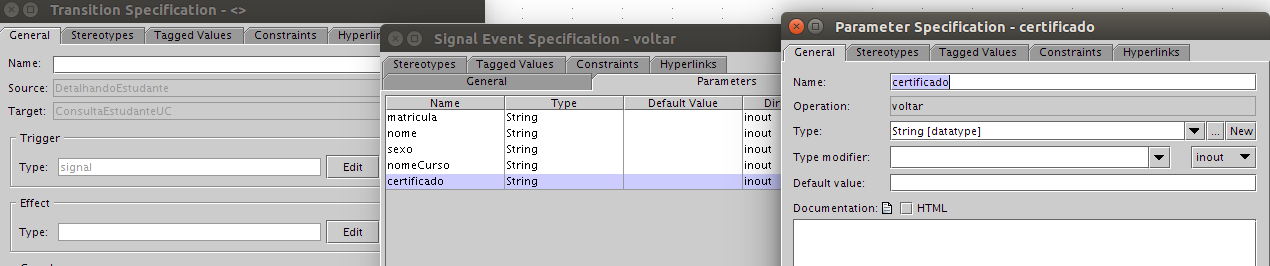
\includegraphics[scale=0.75]{files/imgs/operation-mode-00.png}
	\caption{Criando o campo}
	\label{criando_campo_modo_operacao}
\end{figure}

\item Agora clique na aba Tagged Values:
@andromda.presentation.view.operation.mode.
\item Em seguida clique em Create Value.
\item Agora digite o nova do valor que voce deseja, que no nosso caso será
CERTIFICADO

\begin{figure}[H]
	\centering
	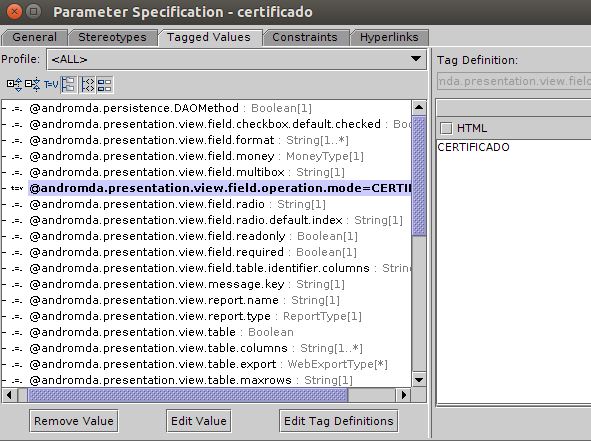
\includegraphics[scale=0.75]{files/imgs/operation-mode-01.png}
	\caption{Adicionando o modo de operação do campo}
	\label{aicionando_modo_operacao_campo}
\end{figure}

\item Pelo Eclipse vá ao ponto de implementação da classe de controle que tem
que disparar o modo de operação e adicione o seguinte código:

\begin{lstlisting}[language=java, frame=single, breaklines=true]
if( estudante.getSexo().getValue().equals("M") ){
	adicionaModoOperacao("CERTIFICADO",container);// <---- Aqui disparamos o MODO OPERACAO
	form.setCertificado(estudante.getCertificado());
}
\end{lstlisting}

\end{enumerate}

Quando chamarmos essa classe de controle, nós iremos invocar o modo de operação
da view caso a condição seja satisfeita nesse caso.

Em seguida, mostraremos como fazer a invocação do modo de operação pelo fluxo.

\subsection{Invocando pelo Fluxo}

Fazendo por fluxo, temos que colocar um valor no valor etiquetado
@andromda.presentation.action.input.operation.mode de uma transição que está
indo para o caso de uso (indo para um estado final) que contém o campo com o
mesmo modo de operação.

\begin{figure}[H]
	\centering
	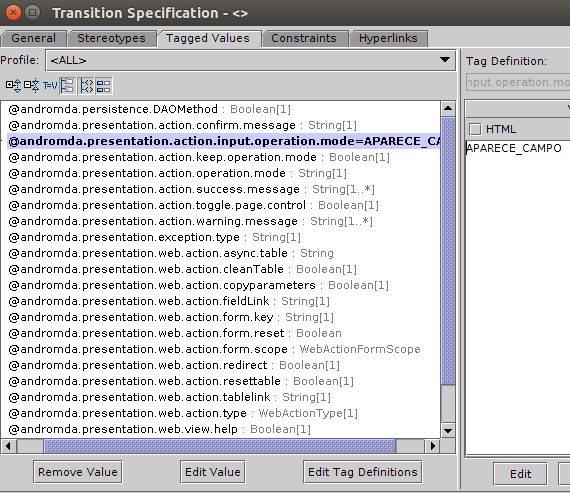
\includegraphics[scale=0.75]{files/imgs/operation-mode-02.png}
	\caption{Adicionando o modo de operação do campo}
	\label{aicionando_modo_operacao_campo}
\end{figure}

Repita o passo 1 da invocação por controlador para ter um campo em que o
funcionamento do modo de operação possa ser testado. Apenas isso precisa ser
feito para fazer modo de operação por fluxo.

Existe um valor no valor etiquetado
@andromda.presentation.action.keep.operation.mode que é também usado em uma
transição que está indo para um estado. Se colocar o valor dele como true você
manterá para o próximo caso de uso o modo de operação recebido de outro caso de
uso.

\subsection{Implementação}

\subsubsection{Sistema}

\subsubsection{Componentes}

\subsection{Na JSP\ldots}

Nas PaginasPersonalizadas, o modo de operação aparece como a tag

<security:containsOperationMode value=“NomeDoModoDeOperacao”>

que envolve o componente definido pelo caso de uso.


\subsection{Regra de ouro do modo de operação}

    Se o componente não possuir nenhum modo de operação definido, ele será
    exibido sempre,  independente se existe ou não um modo de operação definido no sistema.
    
    Se o componente tiver um modo de operação definido,  o componente só será
    exibido na página se o modo de operação do sistema for igual
    
    Você pode definir mais de um modo de operação,  tanto para o sistema quanto
    para um componente. Basta separar os nomes dos modos de operação por vírgula.

